\section{Visualisation}
\label{sec:visualisation}
Every run is turned into an animation with Manim \cite{manim} (\code{src/sim/draw*.py}).
Each video shows the moving body next to live plots of the quantities from \cref{sec:observables}, so the motion and the numbers can be followed together.
The full videos are listed in \ref{app:videos}; this section shows stills from them.

Each script reads a CSV file written by one of the engines, rebuilds the body from the masses and springs listed in its header, and computes the body axes, $\vb*{\Omega}$ and $\vb{L}$ frame by frame as in \cref{sec:observables}.
The playback speed is chosen so that the motion is easy to follow: the octahedron runs are sped up four times, the long damped run twelve times, and the \SI{0.7}{s} racket toss is shown in slow motion.
The videos are rendered at $3840\times2160$ pixels and 60 frames per second.
Seeing the body and the plots side by side also served as a quick check of the simulations, for example that $\vb{L}$ really stays fixed in space while the body turns over.

\Cref{fig:vis-omega,fig:vis-polhode} follow the octahedron spun about its intermediate axis, the first as a still from the video and the second as a plot of $\vb{L}$ seen from the body, made from the same data.
\Cref{fig:vis-racket} shows one toss of a tennis racket computed with the quaternion solver, and \cref{fig:vis-major} shows a damped body moving to its major axis.

\begin{figure*}[tp]
    \centering
    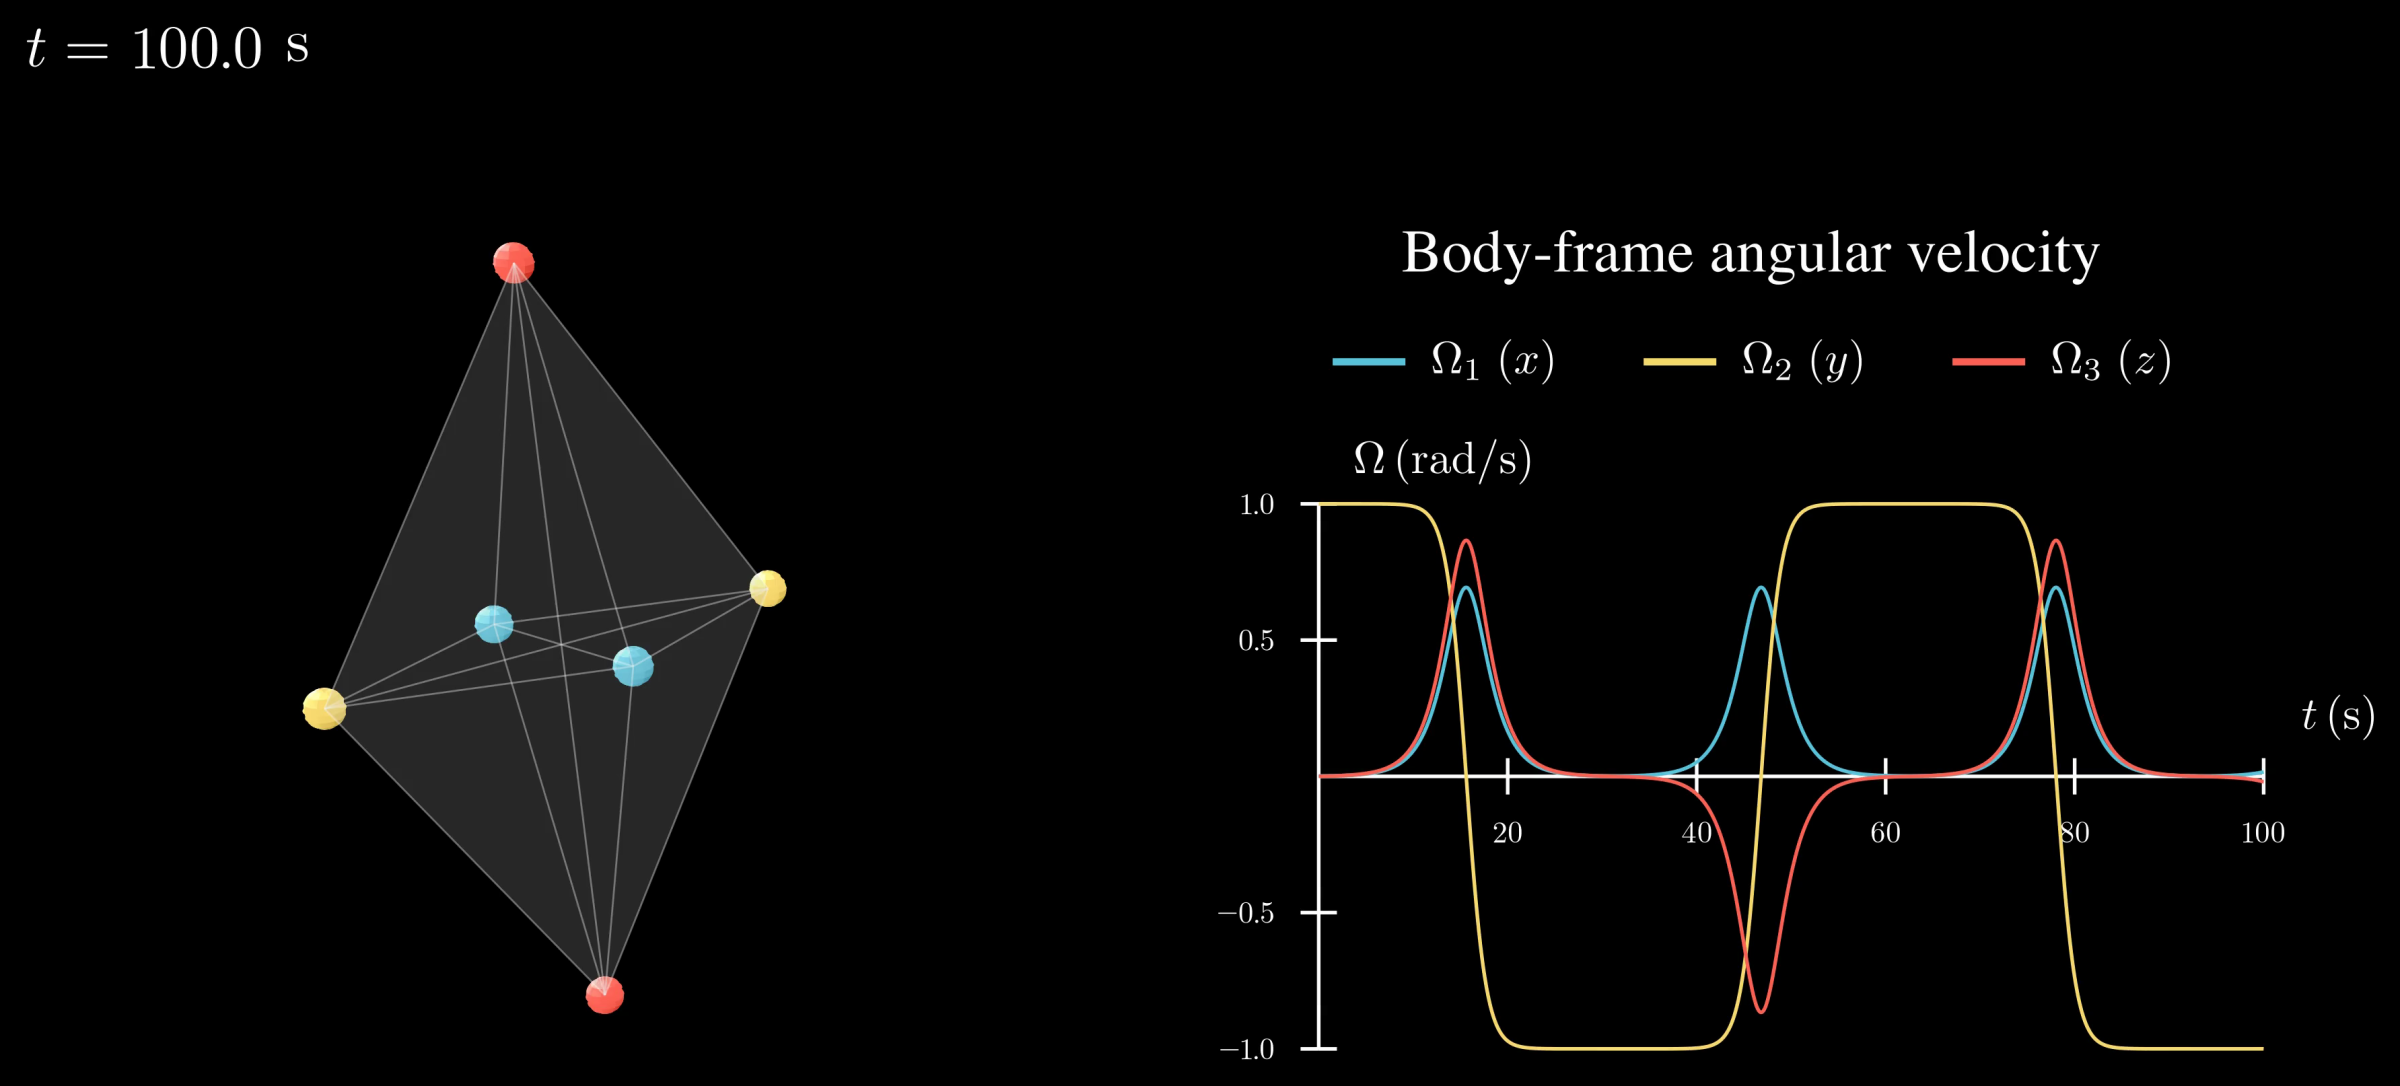
\includegraphics[width=0.9\textwidth]{Images/vis_omega.png}
    \caption{Octahedron (\cref{sec:inertia}) spun at \SI{1}{rad/s} about its intermediate axis $y$ (spring engine, $t=0$--\SI{100}{s}). Left: the body at the end of the run. Right: the body-frame angular velocity. $\Omega_2$ stays almost constant for long stretches and then suddenly reverses sign; each reversal is a flip. During a flip the spin briefly moves into the other two axes, giving the pulses in $\Omega_1$ and $\Omega_3$. The flips repeat regularly, here three times in \SI{100}{s}.}
    \label{fig:vis-omega}
\end{figure*}

\begin{figure*}[tp]
    \centering
    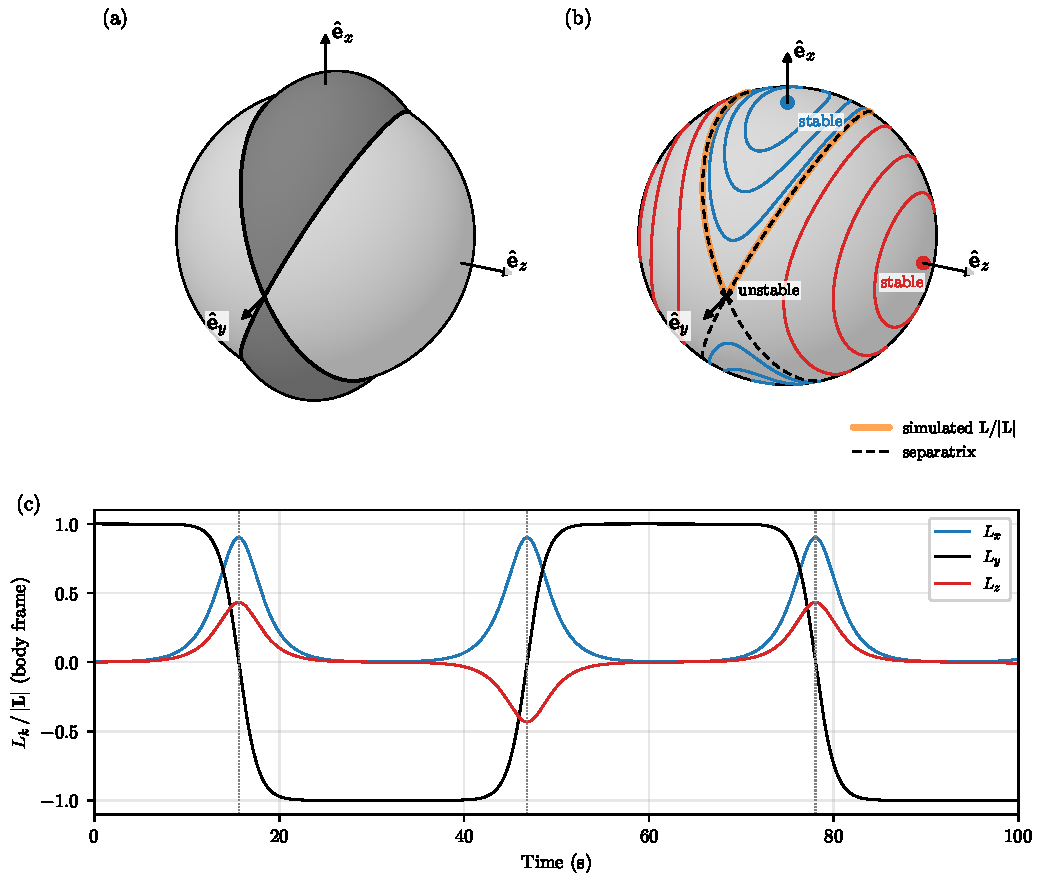
\includegraphics[width=0.75\textwidth]{Images/polhode_sim.pdf}
    \caption{Angular momentum in the body frame for the same run, plotted from the simulation data. (a) The energy ellipsoid of this run (dark grey) cuts the sphere $\abs{\vb{L}}=\text{const}$ (light grey); $\vb{L}$ must stay on the curves where they meet, which here lie almost on the separatrix through the intermediate axis $\vu{e}_y$. (b) Polhodes at other energies: blue curves circle the stable major axis $\vu{e}_x$, red curves the stable minor axis $\vu{e}_z$, and the dashed separatrix crosses at the unstable intermediate axis. The simulated $\vb{L}/\abs{\vb{L}}$ over the whole \SI{100}{s} (orange) runs just beside the separatrix, too close to tell apart here (\cref{sec:analytic}); $2E/L^2$ changes by less than $10^{-5}$ of its value. (c) Body-frame components of $\vb{L}$: $L_y$ jumps between $\pm1$ at each flip (dotted lines, every \SI{31.2}{s}), while $\vb{L}$ passes through the $x$ side of the sphere.}
    \label{fig:vis-polhode}
\end{figure*}

\begin{figure*}[tp]
    \centering
    \begin{minipage}[c]{0.48\textwidth}\centering
        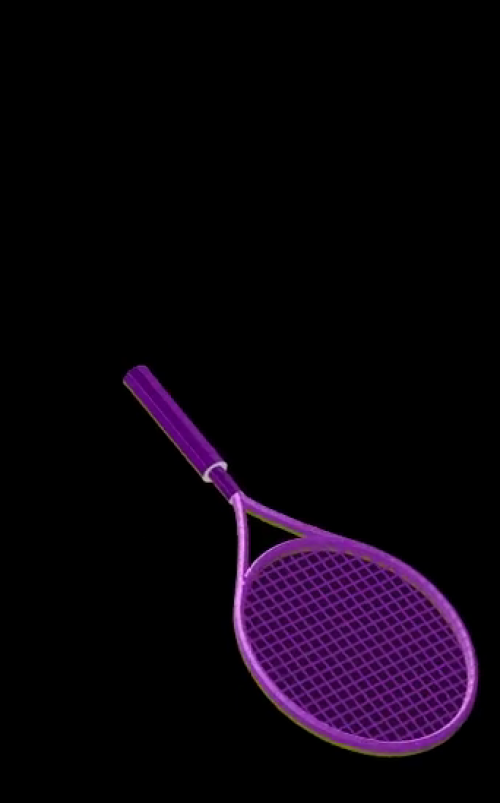
\includegraphics[width=0.32\linewidth]{Images/vis_racket_1.png}\hfill
        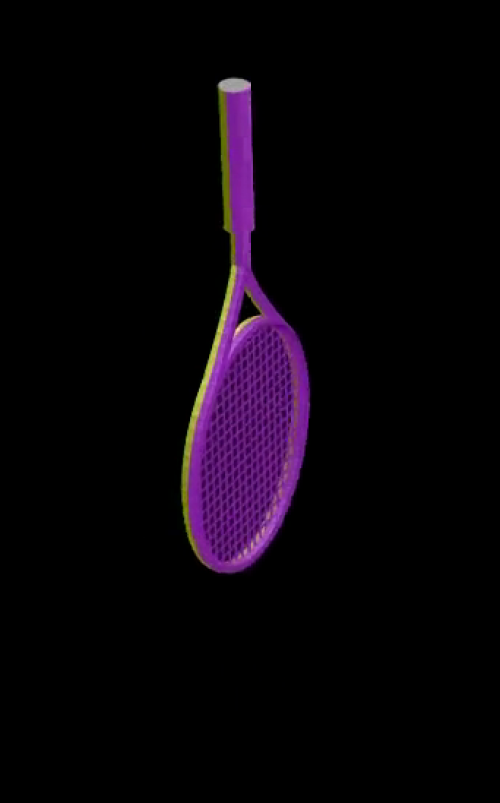
\includegraphics[width=0.32\linewidth]{Images/vis_racket_2.png}\hfill
        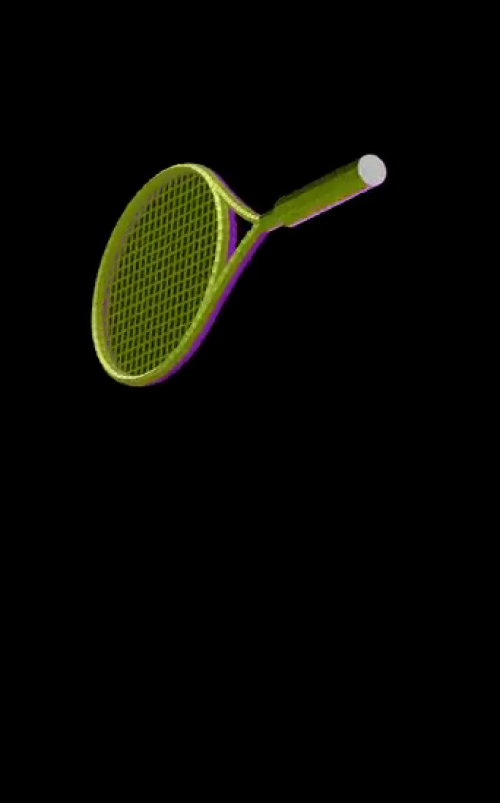
\includegraphics[width=0.32\linewidth]{Images/vis_racket_3.png}\\
        {\footnotesize \makebox[0.32\linewidth]{$t=\SI{0.04}{s}$}\hfill\makebox[0.32\linewidth]{$\SI{0.18}{s}$}\hfill\makebox[0.32\linewidth]{$\SI{0.28}{s}$}}\\[4pt]
        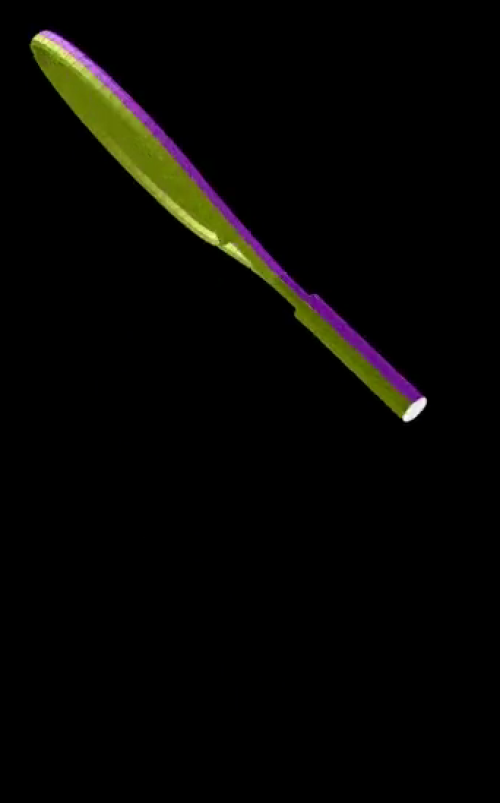
\includegraphics[width=0.32\linewidth]{Images/vis_racket_4.png}\hfill
        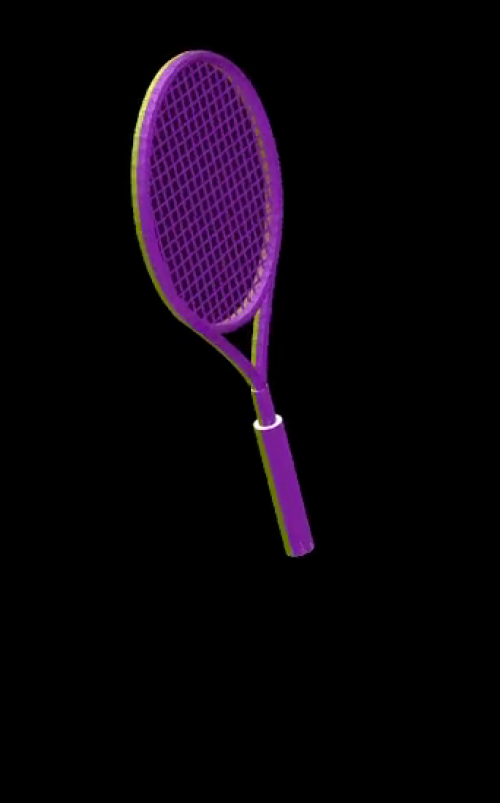
\includegraphics[width=0.32\linewidth]{Images/vis_racket_5.png}\hfill
        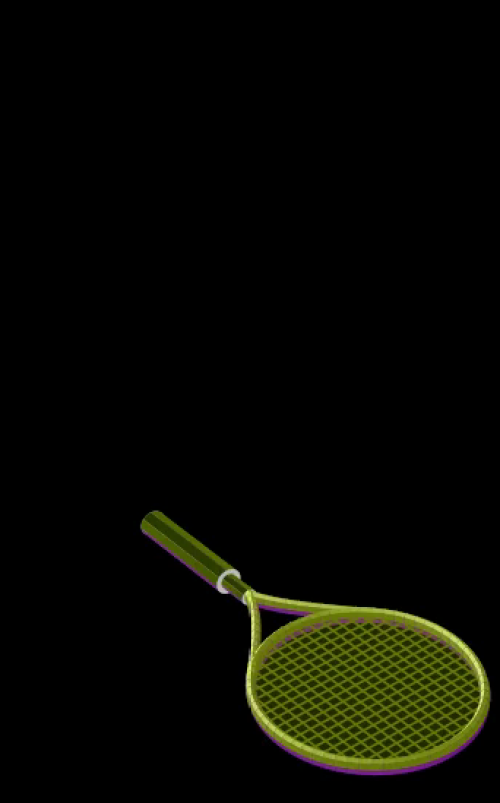
\includegraphics[width=0.32\linewidth]{Images/vis_racket_6.png}\\
        {\footnotesize \makebox[0.32\linewidth]{$\SI{0.40}{s}$}\hfill\makebox[0.32\linewidth]{$\SI{0.52}{s}$}\hfill\makebox[0.32\linewidth]{$\SI{0.70}{s}$}}
    \end{minipage}\hfill
    \begin{minipage}[c]{0.48\textwidth}\centering
        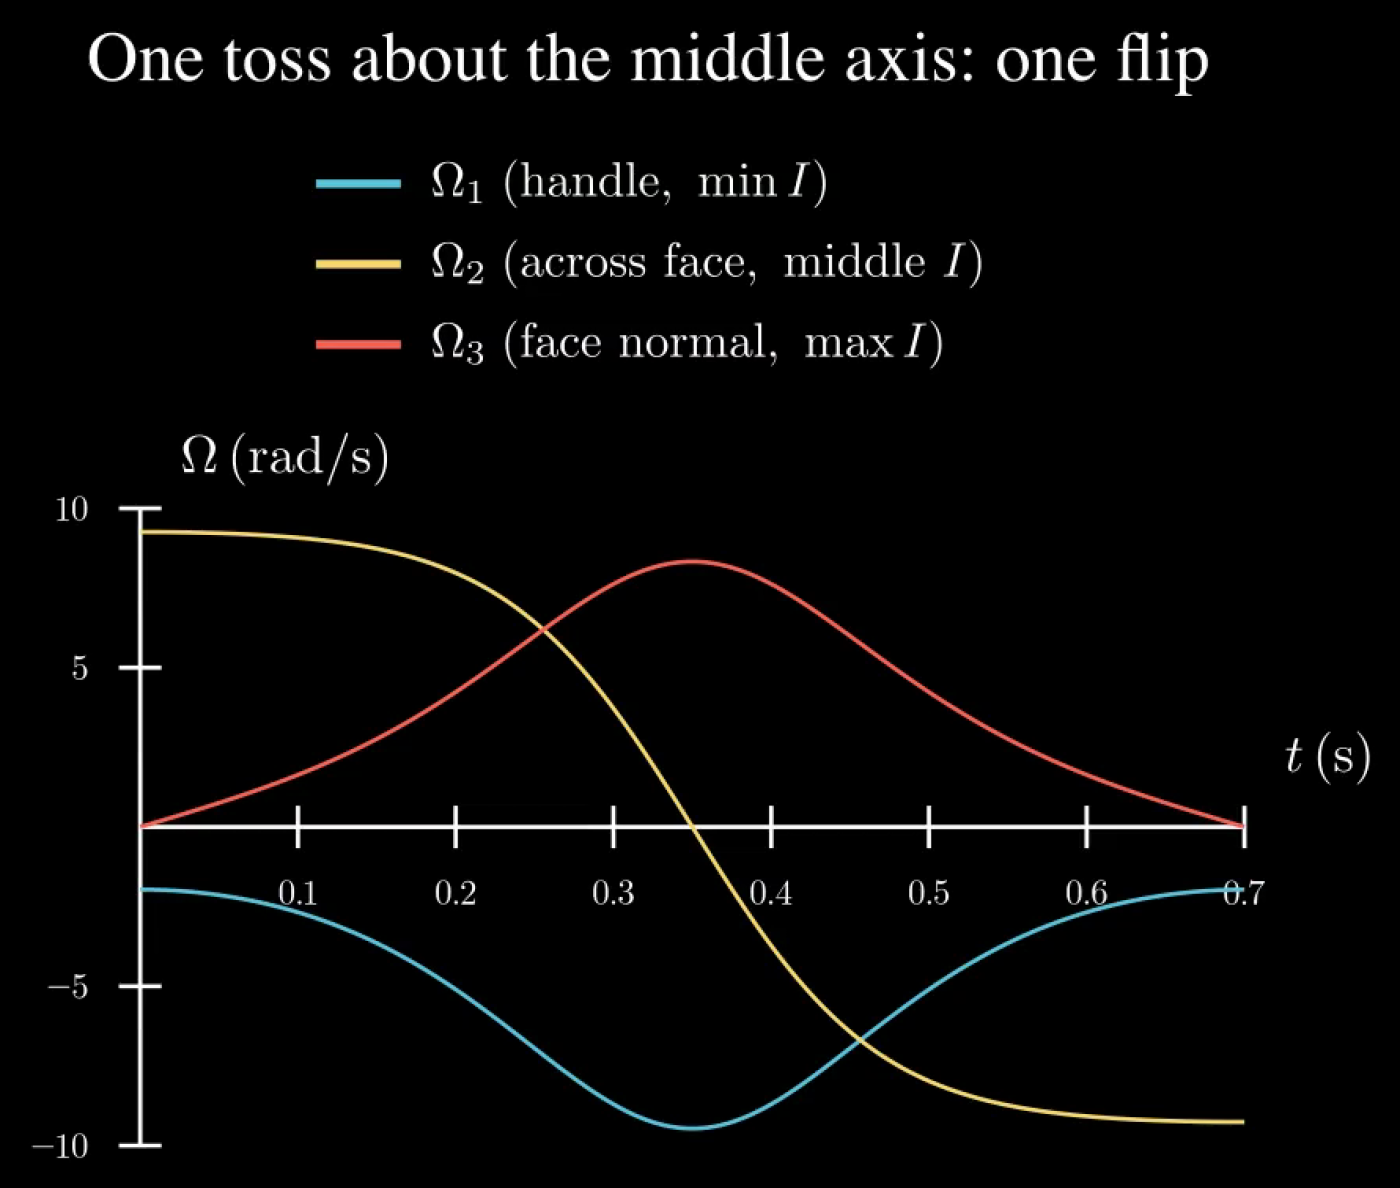
\includegraphics[width=\linewidth]{Images/vis_racket_plot.png}
    \end{minipage}
    \caption{One toss of a tennis racket (\code{quaternion.py}, RK4 with quaternions). The racket is thrown spinning end over end, about its intermediate axis, with a twist about the handle of 21\% of the main spin, which tilts $\vb{L}$ only \ang{1.3} from the intermediate axis. The two sides of the strings are drawn in different colours (purple and yellow). Left: snapshots during the \SI{0.7}{s} flight; the racket comes back with the other side of the face showing, having made a half turn about its handle. Right: the body-frame angular velocity. As $\Omega_2$ (intermediate axis) reverses, the spin passes through the handle ($\Omega_1$) and face-normal ($\Omega_3$) axes, the same pattern as one flip in \cref{fig:vis-omega}.}
    \label{fig:vis-racket}
\end{figure*}

\begin{figure*}[tp]
    \centering
    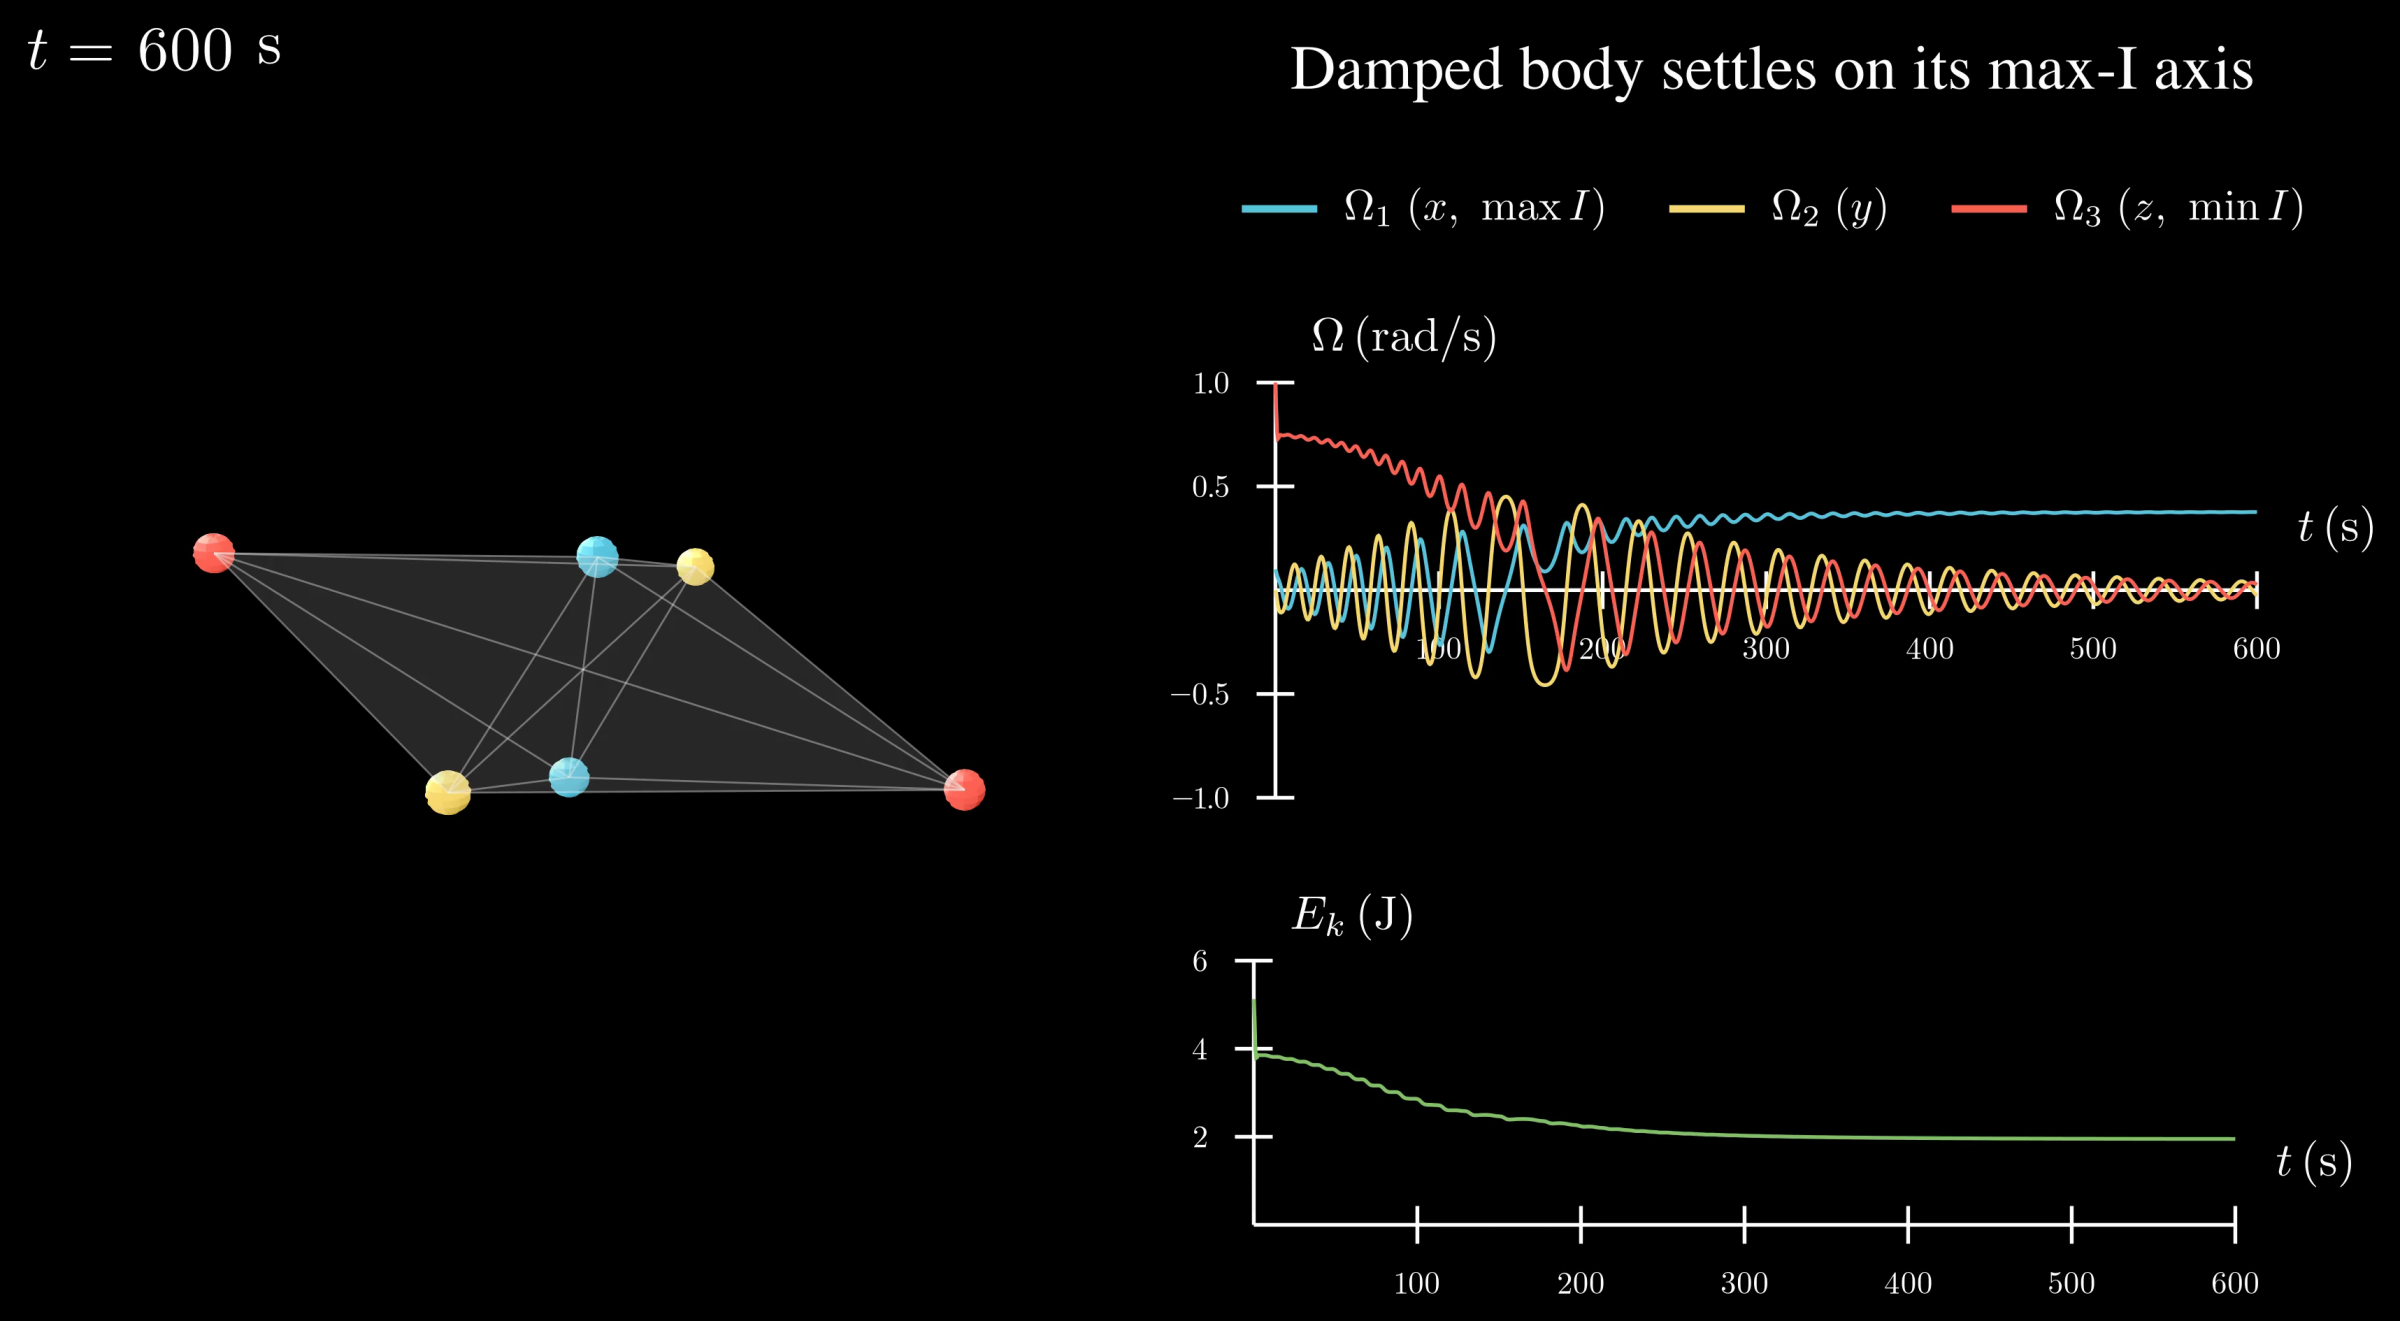
\includegraphics[width=0.8\textwidth]{Images/vis_major_axis.png}
    \caption{A damped body (soft springs, $k=\SI{1}{N/m}$, $c=\SI{0.7}{N.s/m}$) started spinning about its \emph{minor} axis $z$, slightly tilted toward $x$, shown at $t=\SI{600}{s}$. Top right: the spin about $z$ ($\Omega_3$) dies away while the spin about $x$, the major axis, grows and settles. Bottom right: the kinetic energy falls and levels off near $L^2/2I_{\max}\approx\SI{2.0}{J}$, the lowest energy possible at fixed $\vb{L}$ (\cref{sec:res-major}). Even rotation about the minor axis, stable for a rigid body, is not stable once the body can lose energy.}
    \label{fig:vis-major}
\end{figure*}
